\documentclass[aspectratio=169]{beamer}

\usepackage[T1]{fontenc}
\usepackage[utf8]{inputenc}
\usepackage{lmodern}
\usepackage{booktabs}
\usepackage{tabularx}
\usepackage{array}
\usepackage{multirow}
\usepackage{tikz}
\usetikzlibrary{arrows.meta,positioning,fit,backgrounds}
\usepackage{hyperref}

\definecolor{navy}{HTML}{1F3A5F}
\definecolor{teal}{HTML}{1D7A7A}
\definecolor{gold}{HTML}{A67C00}
\definecolor{softbg}{HTML}{F6F8FB}

\hypersetup{
    colorlinks=true,
    linkcolor=navy,
    urlcolor=teal
}

\usetheme{default}
\setbeamertemplate{navigation symbols}{}
\setbeamertemplate{itemize items}[circle]
\setbeamertemplate{sections/subsections in toc}[circle]
\setbeamercolor{structure}{fg=navy}
\setbeamercolor{frametitle}{fg=navy,bg=softbg}
\setbeamercolor{title}{fg=navy}
\setbeamercolor{block title}{fg=white,bg=navy}
\setbeamercolor{block body}{bg=softbg}

\title[NanoBubbleEval]{NanoBubbleEval}
\subtitle{From a large scientific warehouse to a benchmark-ready nanobubble dataset}
\author{Anonymous Authors}
\date{\today}

\newcommand{\yes}{\texttt{yes}}
\newcommand{\nr}{\texttt{NOT\_REPORTED}}

\begin{document}

\begin{frame}
  \titlepage
\end{frame}

\begin{frame}{Project Overview}
\begin{itemize}
    \item We first built a large literature warehouse from public scholarly APIs and curated seed records.
    \item We then tightened the warehouse into a high-precision nanobubble core.
    \item Finally, we formed benchmark-ready subsets for scientific NLP tasks:
    structured extraction, numerical grounding, and evidence attribution.
\end{itemize}
\vspace{0.5em}
\begin{block}{Current status}
\begin{itemize}
    \item Full warehouse: 49,182 deduplicated records
    \item High-precision nanobubble core: 7,785 records
    \item Benchmark candidates: 500 and 1,000 records
\end{itemize}
\end{block}
\end{frame}

\begin{frame}{Workflow Summary}
\centering
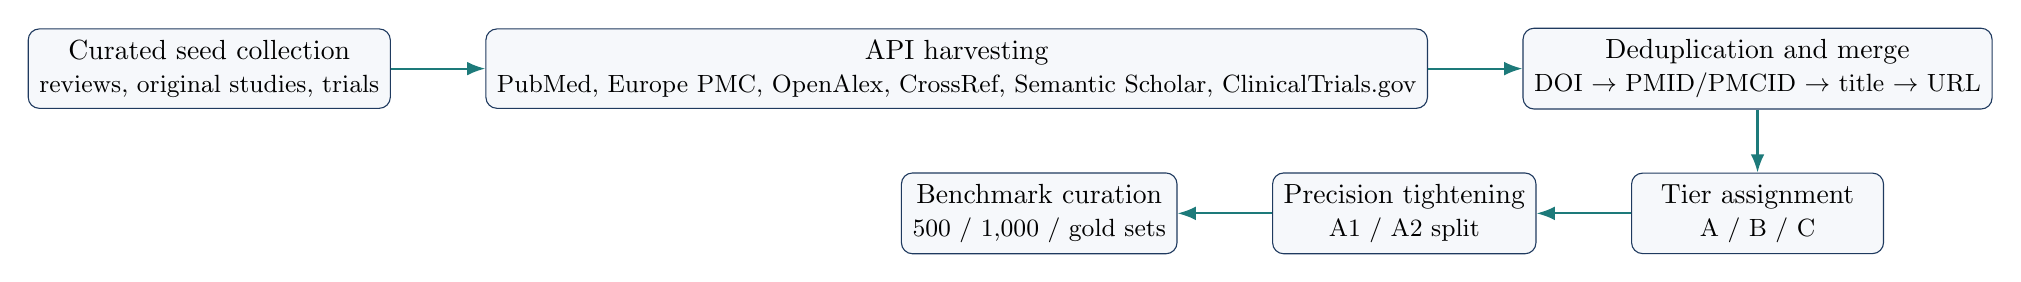
\begin{tikzpicture}[
    node distance=8mm and 12mm,
    box/.style={draw=navy, rounded corners, fill=softbg, align=center, inner sep=4pt, minimum width=3.2cm, minimum height=1cm},
    arrow/.style={-Latex, thick, draw=teal}
]
\node[box] (seed) {Curated seed collection\\\small reviews, original studies, trials};
\node[box, right=of seed] (api) {API harvesting\\\small PubMed, Europe PMC, OpenAlex, CrossRef, Semantic Scholar, ClinicalTrials.gov};
\node[box, right=of api] (dedupe) {Deduplication and merge\\\small DOI $\rightarrow$ PMID/PMCID $\rightarrow$ title $\rightarrow$ URL};
\node[box, below=of dedupe] (tier) {Tier assignment\\\small A / B / C};
\node[box, left=of tier] (precision) {Precision tightening\\\small A1 / A2 split};
\node[box, left=of precision] (bench) {Benchmark curation\\\small 500 / 1,000 / gold sets};

\draw[arrow] (seed) -- (api);
\draw[arrow] (api) -- (dedupe);
\draw[arrow] (dedupe) -- (tier);
\draw[arrow] (tier) -- (precision);
\draw[arrow] (precision) -- (bench);
\end{tikzpicture}
\end{frame}

\begin{frame}{How The Data Was Collected}
\begin{enumerate}
    \item \textbf{Initial seed collection}: We started with curated nanobubble and nanoparticle papers from literature platforms and trial records.
    \item \textbf{API-driven harvesting}: We expanded at scale using structured APIs instead of aggressive page scraping.
    \item \textbf{Query-family expansion}: We ran core nanobubble, adjacent imaging/therapy, delivery, release, and nanocarrier query families.
    \item \textbf{Citation chasing and metadata aggregation}: Review and graph-based sources were used to pull related works and references.
    \item \textbf{Deduplication}: Records were merged by DOI first, then PMID/PMCID, then normalized title, then URL.
    \item \textbf{Tier assignment}: Records were labeled Tier A, B, or C based on lexical and topical proximity.
    \item \textbf{Precision tightening}: Tier A was split into A1 and A2 for nanobubble-core filtering.
    \item \textbf{Benchmark curation}: We built candidate pools and gold-annotation sets from the high-value portion of the warehouse.
\end{enumerate}
\end{frame}

\begin{frame}{APIs and Sources}
\begin{block}{Primary sources}
\begin{itemize}
    \item \textbf{PubMed / NCBI Entrez}: high-volume biomedical metadata and abstracts.
    \item \textbf{Europe PMC}: abstracts, open-access signals, and citation counts.
    \item \textbf{OpenAlex}: large scholarly graph expansion and reference/citation linking.
    \item \textbf{CrossRef}: DOI-centric metadata and venue discovery.
\end{itemize}
\end{block}
\begin{block}{Secondary sources}
\begin{itemize}
    \item \textbf{Semantic Scholar}: citation graph expansion around high-priority works.
    \item \textbf{ClinicalTrials.gov}: translational and clinical trial records.
    \item \textbf{Curated seed records}: a small initial set used to bootstrap expansion.
\end{itemize}
\end{block}
\end{frame}

\begin{frame}{What One Record Contains}
\small
\begin{columns}[T,onlytextwidth]
\column{0.50\textwidth}
\begin{block}{Core metadata}
\begin{itemize}
    \item title
    \item authors
    \item year
    \item journal / venue
    \item DOI
    \item PMID / PMCID if available
    \item URL
    \item source API
    \item document type
    \item access level
\end{itemize}
\end{block}

\column{0.50\textwidth}
\begin{block}{Extraction and curation signals}
\begin{itemize}
    \item tier label
    \item nanobubble vs nanoparticle tag
    \item application category
    \item likely size / zeta / stability / payload / loading / release flags
    \item relevance score
    \item extraction-priority score
    \item notes
    \item placeholders for annotation evidence spans
\end{itemize}
\end{block}
\end{columns}
\end{frame}

\begin{frame}{Dataset Structure}
\begin{tabularx}{\textwidth}{>{\bfseries}p{3.4cm}X}
\toprule
Layer & Description \\
\midrule
Full warehouse & 49,182 deduplicated records spanning nanobubble-core, adjacent nanocarrier, and broader extraction-relevant nanoparticle literature. \\
High-precision core & 7,785 records, split into A1 and A2, used to isolate the cleanest nanobubble-centered material. \\
Benchmark candidates & 500- and 1,000-record balanced subsets designed for model evaluation and manual review. \\
Gold annotation pools & 200 and 500 candidate records ranked for human verification and future expansion. \\
Task packages & Separate files for structured extraction, numerical grounding, and evidence attribution. \\
\bottomrule
\end{tabularx}
\end{frame}

\begin{frame}{Quantitative Summary}
\begin{table}
\centering
\small
\begin{tabular}{lrr}
\toprule
Statistic & Count & Notes \\
\midrule
Full warehouse & 49,182 & deduplicated records \\
High-precision nanobubble core & 7,785 & A1 + A2 \\
A1 & 3,573 & explicit nanobubble core \\
A2 & 4,212 & adjacent ultrasound/gas-carrier \\
Benchmark candidate 500 & 500 & balanced subset \\
Benchmark candidate 1000 & 1,000 & balanced subset \\
Gold annotation set v2 & 200 & manual review pool \\
Gold annotation set v3 & 500 & ranked candidates \\
Structured extraction benchmark & 500 & task package \\
Numerical grounding benchmark & 500 & task package \\
Evidence attribution benchmark & 500 & task package \\
\bottomrule
\end{tabular}
\end{table}
\end{frame}

\begin{frame}{Source, Tier, and Coverage Snapshot}
\begin{columns}[T,onlytextwidth]
\column{0.50\textwidth}
\begin{block}{Source counts}
\begin{itemize}
    \item OpenAlex: 40,836
    \item PubMed: 6,280
    \item Europe PMC: 1,178
    \item CrossRef: 548
    \item Semantic Scholar: 250
    \item ClinicalTrials.gov: 10
    \item Curated seeds: 80
\end{itemize}
\end{block}

\column{0.50\textwidth}
\begin{block}{Coverage}
\begin{itemize}
    \item Records with abstracts: 34,844 (70.8\%)
    \item Records with likely numeric extraction fields: 38,071 (77.4\%)
    \item Tier A: 9,028
    \item Tier B: 8,217
    \item Tier C: 31,937
\end{itemize}
\end{block}
\end{columns}
\end{frame}

\begin{frame}{Field Coverage}
\begin{tabularx}{\textwidth}{lrr}
\toprule
Field & Count & Comment \\
\midrule
Size & 12,838 & comparatively strong \\
Zeta potential & 3,350 & still the weakest field \\
Stability & 9,964 & strong in review and design papers \\
Payload & 27,369 & strongest signal overall \\
Loading efficiency & 9,657 & improved, but still below payload \\
Release profile & 12,462 & common in drug-delivery papers \\
\bottomrule
\end{tabularx}
\vspace{0.6em}
\begin{itemize}
    \item The benchmark is strongest for payload, size, stability, and release-related extraction.
    \item Zeta potential remains the most underrepresented target field.
\end{itemize}
\end{frame}

\begin{frame}{Benchmark Subsets}
\begin{itemize}
    \item \textbf{nanobubble\_core\_high\_precision.csv}: 7,785-record filtered core subset.
    \item \textbf{benchmark\_candidate\_500.csv}: compact, balanced evaluation slice.
    \item \textbf{benchmark\_candidate\_1000.csv}: larger candidate pool for manual curation and benchmarking.
    \item \textbf{gold\_annotation\_set\_v2.csv}: 200-record manual annotation pool.
    \item \textbf{gold\_annotation\_set\_v3.csv}: 500-ranked candidate pool.
    \item \textbf{structured\_extraction\_benchmark.csv}: schema-filling task package.
    \item \textbf{numerical\_grounding\_benchmark.csv}: numeric value extraction and normalization package.
    \item \textbf{evidence\_attribution\_benchmark.csv}: supporting-span identification package.
\end{itemize}
\end{frame}

\begin{frame}{Why This Matters for NeurIPS}
\begin{itemize}
    \item The warehouse is large enough to support robust corpus statistics and benchmark design.
    \item The benchmark is domain-specific but still broad enough to test general scientific NLP capabilities.
    \item The tasks require structured extraction, numerical grounding, and evidence attribution rather than shallow classification.
    \item The data includes review papers, original studies, translational records, and clinically relevant signals.
    \item The project can support both automatic evaluation and manually verified gold benchmarking.
\end{itemize}
\end{frame}

\begin{frame}{Strengths and Current Limitations}
\begin{block}{Strengths}
\begin{itemize}
    \item Large deduplicated warehouse with rich metadata.
    \item Explicit tiering and benchmark curation logic.
    \item Strong coverage for payload, size, stability, and release profile.
    \item Reproducible API-first collection workflow.
\end{itemize}
\end{block}
\begin{block}{Limitations}
\begin{itemize}
    \item Tier C is broad and intentionally mixed.
    \item ClinicalTrials.gov coverage is still small.
    \item Zeta potential is weaker than payload and size.
    \item Some records are metadata-rich but not full-text rich.
    \item The A1 precision proxy is heuristic, not a gold-standard annotation score.
\end{itemize}
\end{block}
\end{frame}

\begin{frame}{Questions My Supervisor May Ask}
\begin{block}{Why 49K records but only 7.7K in the high-precision core?}
The warehouse is intentionally broad. The 7,785-record core keeps only the clearest nanobubble-centered records, while the rest of the warehouse supports context, adjacent methods, and benchmark diversity.
\end{block}
\begin{block}{What is the difference between warehouse and benchmark?}
The warehouse is the full deduplicated literature bank. The benchmark is a curated subset chosen for evaluation, annotation, and task design.
\end{block}
\begin{block}{Why is A1 more trustworthy?}
A1 requires strong explicit nanobubble lexical evidence, so it is less likely to contain broad nanoparticle-only records.
\end{block}
\begin{block}{What exactly is inside one record?}
Metadata, source provenance, tier label, nanobubble/nanoparticle tag, likely extraction fields, scores, and placeholders for evidence spans and reviewer notes.
\end{block}
\begin{block}{What are the next steps toward publication?}
Finalize the annotation guide, manually verify gold records, run baseline extractors, and evaluate structured extraction, numerical grounding, and evidence attribution.
\end{block}
\end{frame}

\begin{frame}{Next Steps}
\begin{enumerate}
    \item Finalize the annotation guide and decision rules.
    \item Manually verify the 200- and 500-record gold pools.
    \item Run baseline extraction systems on the benchmark packages.
    \item Report structured extraction, numerical grounding, and evidence attribution metrics.
    \item Prepare the paper with dataset, workflow, and benchmark sections.
\end{enumerate}
\end{frame}

\end{document}

\section{Dataset Splits}
A convincing benchmark should not rely only on random splits.

\subsection{Random Split}
For initial experiments.

\subsection{Temporal Split}
Train on older literature and test on newer studies.

\subsection{Source Split}
Train on some platforms or publishers and test on others where feasible.

\subsection{Document-Type Split}
Separate review papers, original research articles, and clinical-study summaries.

\subsection{Evidence-Type Split}
Compare prose-heavy versus table-heavy documents.

\section{Baseline Systems}
The benchmark should evaluate multiple baseline categories.

\subsection{Rule-Based Baselines}
Pattern matching and regex pipelines for size, zeta potential, and other numeric properties.

\subsection{Encoder-Based Baselines}
Scientific span extraction models or sequence labeling systems.

\subsection{LLM-Based Baselines}
Instruction-following models prompted to produce schema-constrained JSON outputs.

\subsection{Retrieval-Augmented Baselines}
Chunk retrieval followed by evidence-grounded extraction.

\section{Anticipated Failure Modes}
The paper should include a formal error taxonomy. Likely failure modes include:
\begin{itemize}[leftmargin=2em]
    \item hallucinated quantitative values,
    \item wrong unit interpretation,
    \item confusion between payload and release information,
    \item mixing nanobubble and nanoparticle descriptions,
    \item weak grounding to evidence spans,
    \item inability to recover values from tables,
    \item incorrect association of values with the wrong experimental context.
\end{itemize}

\section{Annotation Workflow}
\subsection{Step 1: Corpus Collection}
Collect papers from the identified sources.

\subsection{Step 2: Review-Based Prioritization}
Use review papers to define core terminology, recurring variables, and important experimental categories.

\subsection{Step 3: Pilot Annotation}
Annotate a small sample to refine schema definitions and evidence-labeling rules.

\subsection{Step 4: Full Annotation}
Expand annotation after agreement and ambiguity issues are resolved.

\subsection{Step 5: Quality Assurance}
Perform adjudication, error checking, and consistency analysis.

\section{Paper Structure}
The final paper can follow this structure.

\subsection{1. Introduction}
Introduce the challenge of scientific information extraction from nanobubble and related literature.

\subsection{2. Background and Motivation}
Discuss domain complexity, literature heterogeneity, and the need for evidence-grounded evaluation.

\subsection{3. Dataset Construction}
Describe collection sources, inclusion criteria, annotation schema, and evidence linking.

\subsection{4. Benchmark Tasks}
Define extraction, numerical grounding, evidence attribution, and cross-document reasoning tasks.

\subsection{5. Experimental Setup}
Present baseline systems, evaluation metrics, and dataset splits.

\subsection{6. Results}
Show task performance, slice-based evaluation, and source/document-type analysis.

\subsection{7. Error Analysis}
Analyze frequent system failures in extracting size, zeta potential, stability, payload, and release-related information.

\subsection{8. Discussion}
Explain what the results reveal about current scientific NLP systems.

\subsection{9. Limitations and Ethics}
Discuss domain scope, annotation subjectivity, data availability, access limitations, and release considerations.

\section{Execution Plan}
\subsection{Phase 1: Scope Definition}
\begin{itemize}[leftmargin=2em]
    \item finalize research framing,
    \item finalize initial search keywords,
    \item define inclusion and exclusion criteria.
\end{itemize}

\subsection{Phase 2: Source Collection}
\begin{itemize}[leftmargin=2em]
    \item gather papers from Google Scholar, ScienceDirect, Springer, and Wiley,
    \item inspect ClinicalTrials.gov for relevant related studies,
    \item organize metadata in a master spreadsheet.
\end{itemize}

\subsection{Phase 3: Schema Finalization}
\begin{itemize}[leftmargin=2em]
    \item finalize fields such as size, zeta potential, stability, payload, and loading-release,
    \item define normalization rules,
    \item finalize evidence-linking policy.
\end{itemize}

\subsection{Phase 4: Pilot Annotation}
\begin{itemize}[leftmargin=2em]
    \item annotate a small subset,
    \item refine edge cases,
    \item compute preliminary agreement.
\end{itemize}

\subsection{Phase 5: Full Dataset Construction}
\begin{itemize}[leftmargin=2em]
    \item annotate the main corpus,
    \item validate records,
    \item prepare benchmark splits.
\end{itemize}

\subsection{Phase 6: Benchmarking}
\begin{itemize}[leftmargin=2em]
    \item implement baselines,
    \item run extraction experiments,
    \item evaluate grounding and numerical correctness.
\end{itemize}

\subsection{Phase 7: Writing and Packaging}
\begin{itemize}[leftmargin=2em]
    \item prepare paper draft,
    \item create dataset documentation,
    \item organize release materials.
\end{itemize}

\section{Suggested Timeline}
\begin{longtable}{p{0.18\textwidth} p{0.72\textwidth}}
\toprule
\textbf{Week} & \textbf{Planned Work} \\
\midrule
Week 1 & Finalize task framing, search strategy, and schema draft \\
Week 2 & Collect review papers and build initial paper inventory \\
Week 3 & Expand to original articles and related nanoparticle literature \\
Week 4 & Finalize structured fields and pilot annotation guide \\
Week 5 & Pilot annotation and ambiguity resolution \\
Week 6--7 & Full data extraction and evidence linking \\
Week 8 & Build baseline systems and evaluation scripts \\
Week 9 & Run experiments and create result tables \\
Week 10 & Perform failure analysis and benchmark interpretation \\
Week 11 & Write the paper draft \\
Week 12 & Revise, package, and prepare release materials \\
\bottomrule
\end{longtable}

\section{Immediate Next Step}
The first practical next step should be:
\begin{quote}
\textit{Create a seed list of review papers and original studies from Google Scholar, ScienceDirect, Springer, and Wiley, then design a pilot annotation sheet focused on size, zeta potential, stability, payload, and loading-release information.}
\end{quote}

\section{Draft Contribution Statement}
A possible contribution statement for later paper writing is:

\begin{quote}
We introduce a literature-grounded evaluation benchmark for scientific information extraction in nanobubble and related nanoscale studies. The benchmark is constructed from publicly accessible scientific literature and emphasizes structured extraction of experimentally important properties such as size, zeta potential, stability, payload, and loading-release behavior. Using this dataset artifact, we evaluate the reliability of modern NLP systems on evidence-grounded scientific extraction and show that current models remain limited in numerical grounding, evidence attribution, and cross-document scientific reasoning.
\end{quote}

\section{Conclusion}
This project is strongest when framed as an \textbf{evaluation study supported by a structured dataset artifact}. The advice received points to a clear and practical starting point: begin from review papers and major scientific databases, extract quantitative scientific variables, and organize them into a reproducible benchmark. This creates a realistic path toward a publishable dataset-and-evaluation paper in scientific NLP.

\end{document}
